
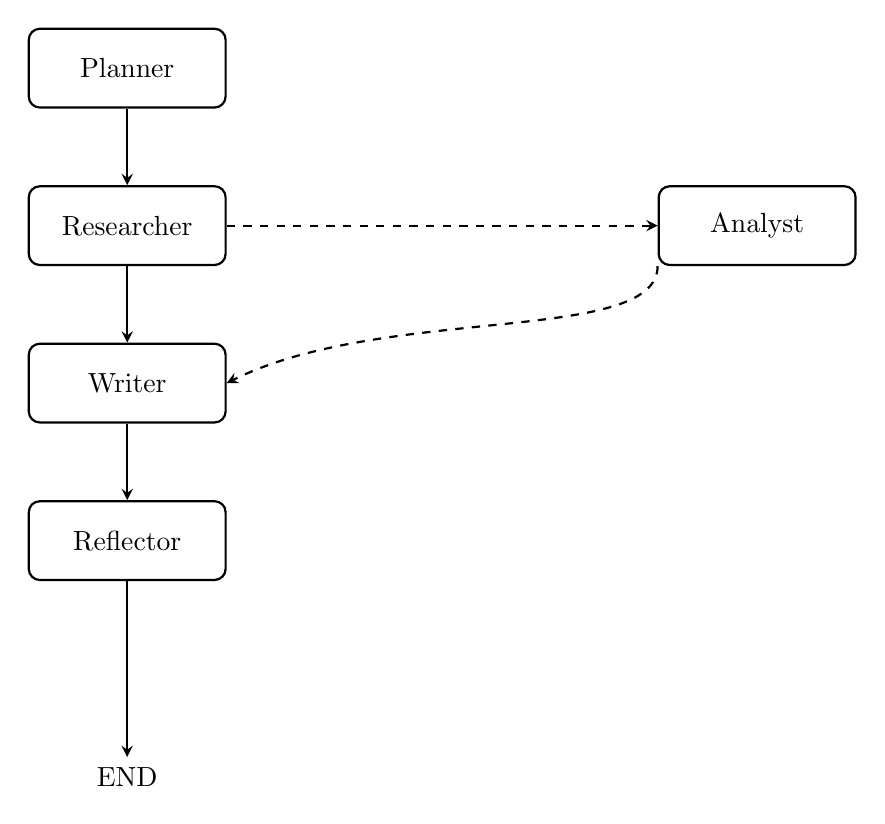
\begin{tikzpicture}[node distance=2cm,>=stealth,thick]
\tikzstyle{node}=[rectangle,draw,rounded corners,minimum width=2.5cm,minimum height=1cm]

\node[node] (planner) {Planner};
\node[node,below of=planner] (researcher) {Researcher};
\node[node,below of=researcher] (writer) {Writer};
\node[node,below of=writer] (reflect) {Reflector};
\node[below of=reflect,yshift=-1cm] (end) {END};

\draw[->] (planner) -- (researcher);
\draw[->] (researcher) -- (writer);
\draw[->] (writer) -- (reflect);
\draw[->] (reflect) -- (end);

% Analyst 分支
\node[node,right of=researcher,xshift=6cm] (analyst) {Analyst};
\draw[->,dashed] (researcher.east) -- (analyst.west);
\draw[->,dashed] (analyst.south west) .. controls +(0,-1) and +(2,1) .. (writer.east);
\end{tikzpicture}
